\documentclass[11pt]{article}
\setlength{\oddsidemargin}{0in}
\setlength{\evensidemargin}{0in}
\setlength{\textwidth}{6.5in}

\usepackage{fancyhdr}
\pagestyle{fancy}
\usepackage{amsmath,amsfonts,amssymb}
\usepackage{epsfig}
\usepackage{subfigure}
\usepackage{placeins}
\usepackage{amsmath}
\usepackage[usenames,dvipsnames,svgnames,table]{xcolor}
\usepackage{amssymb}
\usepackage{setspace}
\usepackage{graphicx} % Include figure files
\usepackage{times}
\usepackage{amsthm}
\usepackage{hyperref}
\usepackage{enumitem}
\hypersetup{bookmarks=true, unicode=false, pdftoolbar=true, pdfmenubar=true, pdffitwindow=false, pdfstartview={FitH}, pdfcreator={Daniel Larremore}, pdfproducer={Daniel Larremore}, pdfkeywords={} {} {}, pdfnewwindow=true, colorlinks=true, linkcolor=blue, citecolor=Green, filecolor=magenta, urlcolor=cyan,}
\usepackage[parfill]{parskip}

\graphicspath{{../Notes/PythonFigs/}{./}}

% styling for solution blocks
\newenvironment{solution}{\par\noindent\begingroup\color{Blue}\textbf{Solution:} }{\par\endgroup}

\newcommand{\e}{\mathrm{e}}
\renewcommand{\d}{\mathrm{d}}
\newcommand{\erf}{\mathop\mathrm{erf}}
\newcommand{\erfc}{\mathop\mathrm{erfc}}
\newcommand{\xmin}{\ensuremath{x_{\min}}}
\newcommand{\ntail}{\ensuremath{n_{\rm tail}}}

\newcommand{\Q}[1]{\footnote{\textcolor{blue}{#1}}}

\begin{document}

\lhead{{\bf Mathematical \& Computational Modeling of Infectious Diseases \\ 
Homework 3}}
\rhead{{\bf D.B.\ Larremore\\2025}}
\renewcommand{\headrulewidth}{0.4pt}

{\bf Instructions:} 
\begin{itemize}[itemsep=-7pt]
	\item Please turn in a single PDF file. 
	\item Please share a link to your code, but do not attach the actual code. 
	\item Handwritten math (scanned and included in a PDF) is fine, but please watch out for 10MB+ file sizes!
\end{itemize}

\vspace{0.1in}\hrule

\begin{enumerate}

\item The goal of this problem is to explore the preferential depletion of susceptibles. 

Consider a population with four equal-sized groups, numbered $1, 2, 3, 4$. Suppose that the contact structure in the population is fully mixed (i.e. $c_{ij} = \bar{c}$ for all $i,j$), that $\gamma_i = 3$ for all $i$, and that $R_0=1.5$, under SIR dynamics. Finally, suppose that the susceptibility for group $1$ is $p_1=1$, the susceptibility for group $2$ is $p_2=2$, with $p_3 = 3$ and $p_4=4$. 

\begin{enumerate}[label=\alph*.]
	\item In terms of $\bar{c}$, $s_1$, $s_2$, $s_3$, and $s_4$ (and constants), what is the next-generation matrix for this system?
	    \begin{solution}
			 With four groups, the matrix will be $4 \times 4$.
			 The NGM can be modeled as follows: 
				\[
				M_{ij} = {\frac{4\bar{c}}{3}}\begin{bmatrix}
				1 s_1 & 1 s_1 & 1 s_1 & 1 s_1 \\
				2 s_2 & 2 s_2 & 2 s_2 & 2 s_2 \\
				3 s_3 & 3 s_3 & 3 s_3 & 3 s_3 \\
				4 s_4 & 4 s_4 & 4 s_4 & 4 s_4 
				\end{bmatrix}
				\]
		\end{solution}
	\item To ensure that $R_0=1.5$, what must $\bar{c}$ be equal to?
	    \begin{solution}
			 To find $\bar{c}$, we need to find the dominant eigenvalue of the NGM. 
			 The dominant eigenvalue is given by:
			 \[
			 \lambda = \frac{4\bar{c}}{3} (1 s_1 + 2 s_2 + 3 s_3 + 4 s_4)
			 \]
			 Assuming disease-free equilibrium, $s_i = 1$ for all $i$.
			 \[
			 \lambda = \frac{4\bar{c}}{3} (1 + 2 + 3 + 4) = \frac{40\bar{c}}{3}
			 \]
			 Solving for $\bar{c}$ with $\lambda = R_0 = 1.5$:
			 \[
			 0.1125 = \bar{c}
			 \]
			 In more mathy terms, to ensure $R_0 = 1.5$, we need:
			 \[
			 \bar{c} = \frac{3 R_0}{40}
			 \]
		\end{solution}
	\item Using these parameters, code up a version of your model with initial conditions where $99.9\%$ of people in each group are susceptible, and the other $0.1\%$ are infected.\footnote{You'll have to modify your code to cope with the fact that there are now 4 groups!} Simulate an epidemic wave using an appropriate timestep $\Delta t$ and appropriate maximum simulation time to capture the wave. Create a plot of the four populations' $I$ compartments vs time, showing $i_1(t)$, $i_2(t)$, $i_3(t)$, and $i_4(t)$. Color these curves in a single hue, but with varying levels of light/dark or saturation, such that the boldest and darkest line is the most susceptible group, and the faintest and lightest line is the least susceptible group.
		\begin{solution}
			\href{https://github.com/JasonHunter95/infectious-diseases/blob/main/HW3/homework_3.ipynb} {My code for this graph}
			\begin{center}
				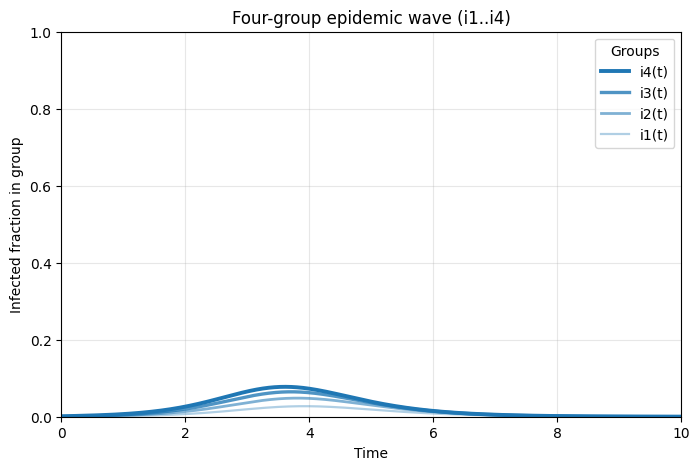
\includegraphics[width=0.7\textwidth]{fourgroups.png}
			\end{center}
		\end{solution}
	\item Define the average relative susceptibility among the susceptibles at any point in time $\bar{p}(t)$ as
%	$$\bar{p}(t) = \frac{\displaystyle \sum_{i=1}^4 p_i\,s_i(t)}{\displaystyle \sum_{i=1}^4 s_i(t)}\ .$$
	$$\bar{p}(t) = \displaystyle \sum_{i=1}^4 p_i\,s_i(t) \Bigg / \displaystyle \sum_{i=1}^4 s_i(t)\ .$$
	Note that this is simply a weighted average of the susceptibilities of the susceptibles, by adding up the susceptibilities in the numerator and dividing by the number of susceptibles in the denominator. Over the same time window as your previous plot, create two addition figures: First, show $s_i(t)$ for each $i=1, 2, 3, 4$ using the same color scheme as before. Second, show $\bar{p}(t)$ in black. 
	\item Comment on what you observe in the plots, and explain the reason for the patterns in words that a high school student could understand.
	\item[Grad/EC] Reflect on these plots in the context of the COVID-19 pandemic. What lessons are there to be drawn from the relationship between an epidemic wave and different groups with different susceptibilities?
\end{enumerate}
\clearpage

\item The goal of this problem is to explore branching processes, and how superspreading can, perhaps surprisingly, increase the likelihood that an outbreak never grows to a large size.

This problem introduces the {\bf negative binomial} (NB) distribution. The distribution can be parameterized a few different ways, but for our purposes, it will be convenient to specify a mean and a dispersion. In the context of transmission chains and branching processes, drawing the number of secondary infections from a negative binomial requires that the mean be $R_0$. However, the dispersion parameter allows us flexibility, and importantly, allows us to model superspreading. 

When $k \to \infty$, the negative binomial distribution converges to a Poisson distribution. When $k = 1$, the negative binomial is equivalent to a geometric distribution. A key difference between these is that the mode of a Poisson---its most common value---is around its mean, while the mode of a Geometric is zero. In the context of branching processes, this means that a high $k$ will lead to more similar numbers of secondary infections for each primary infection. In contrast, a low $k$ will lead to many instances where there are just a few (or zero) secondary infections, and rare instances with a large number of secondary infections. When $k$ is low, we often talk about ``superspreaders,'' people whose infections lead to an exceptionally larger number of secondary infections. 

Note: You can find Python code to draw from a negative binomial with the $R_0$ and $k$ parameterization provided on the next page. For those writing in other languages, be careful to use the correct parameterization (mean and dispersion).

\begin{enumerate}[label=\alph*.]
	\item Write code for a branching process that, starting from a single infection, draws $G$ generations, with each infection creating $NB(R_0,k)$ additional infections. Use your code to estimate $q$ the probability\footnote{See class notes.} that an epidemic dies in finite time, for $R_0=3$ and $k=0.1, 0.5, 1.0, 5.0,$ and $10.0$.\footnote{Hint: When we estimate a probability from a stochastic process like this, a convenient way to do this is Monte Carlo: simulate, say, $100,000$ branching processes and take note of how many cease before growing large.} Provide your answers in a table, out to 3 decimal places.
	\item How does $k$ affect $q$? Explain what this means in terms of the relationship between $p$ (i.e., $1-q$) and superspreading. 
	\item [Grad/EC] How large do finite outbreaks get before they die out? For the parameters above, and for only the {\it finite} outbreaks, plot a histogram of $100,000$ finite outbreaks for your choice or choices of $k$, and $R_0=3$. What do you observe? 
\end{enumerate}

\clearpage
Here is some Python code to draw from $NB(R_0, k)$:
\begin{verbatim}
from scipy.stats import nbinom

k = 10000 # Dispersion Parameter k
R0 = 3 # Mean R0

mean = R0
variance = mean + (mean**2)/k
p = mean/variance
n = mean**2 / (variance - mean) 

draw = nbinom.rvs(n=n,p=p)
draws = nbinom.rvs(n=n,p=p,size=10)
\end{verbatim}



\end{enumerate}

\end{document}